%This is a slight variation of the "sig-alternate.tex". We have added a
%\selfcite{myref} command to the sig-alternate.cls file and some explanations to
%the sig-alternate.tex file. Thus, sig-alternate.cls has been renamed to
%dads.cls and sig-alternate.tex has been renamed to dads[nn].tex

% This is "sig-alternate.tex" V1.9 April 2009
% This file should be compiled with V2.4 of "sig-alternate.cls" April 2009
%
% This example file demonstrates the use of the 'sig-alternate.cls'
% V2.4 LaTeX2e document class file. It is for those submitting
% articles to ACM Conference Proceedings WHO DO NOT WISH TO
% STRICTLY ADHERE TO THE SIGS (PUBS-BOARD-ENDORSED) STYLE.
% The 'sig-alternate.cls' file will produce a similar-looking,
% albeit, 'tighter' paper resulting in, invariably, fewer pages.
%
% ----------------------------------------------------------------------------------------------------------------
% This .tex file (and associated .cls V2.4) produces:
%       1) The Permission Statement
%       2) The Conference (location) Info information
%       3) The Copyright Line with ACM data
%       4) NO page numbers
%
% as against the acm_proc_article-sp.cls file which
% DOES NOT produce 1) thru' 3) above.
%
% Using 'sig-alternate.cls' you have control, however, from within
% the source .tex file, over both the CopyrightYear
% (defaulted to 200X) and the ACM Copyright Data
% (defaulted to X-XXXXX-XX-X/XX/XX).
% e.g.
% \CopyrightYear{2007} will cause 2007 to appear in the copyright line.
% \crdata{0-12345-67-8/90/12} will cause 0-12345-67-8/90/12 to appear in the copyright line.
%
% ---------------------------------------------------------------------------------------------------------------
% This .tex source is an example which *does* use
% the .bib file (from which the .bbl file % is produced).
% REMEMBER HOWEVER: After having produced the .bbl file,
% and prior to final submission, you *NEED* to 'insert'
% your .bbl file into your source .tex file so as to provide
% ONE 'self-contained' source file.
%
% ================= IF YOU HAVE QUESTIONS =======================
% Questions regarding the SIGS styles, SIGS policies and
% procedures, Conferences etc. should be sent to
% Adrienne Griscti (griscti@acm.org)
%
% Technical questions _only_ to
% Gerald Murray (murray@hq.acm.org)
% ===============================================================
%
% For tracking purposes - this is V1.9 - April 2009

\documentclass{dads}   %Changed for DADS

\usepackage{algpseudocode}
\usepackage{algorithm}
\usepackage{amsmath}
\usepackage{amssymb}

\begin{document}
% --- Author Metadata here ---
\conferenceinfo{SAC'19}{April 8--12, 2019, Limassol, Cyprus}
\CopyrightYear{2019} % Allows default copyright year (200x) to be over-ridden - IF NEED BE.
%\crdata{0-12345-67-8/90/01}  % Allows default copyright data (0-89791-88-6/97/05) to be over-ridden - IF NEED BE.
% --- End of Author Metadata ---

\title{Bitshield \titlenote{(Produces the permission block, and
copyright information). For use with
SIG-ALTERNATE.CLS. Supported by ACM.}}

\subtitle{Adaptive information dissemination in the Bitcoin network
%\titlenote{A full version of this paper is available as
%\textit{Author's Guide to Preparing ACM SIG Proceedings Using
%\LaTeX$2_\epsilon$\ and BibTeX} at
%\texttt{www.acm.org/eaddress.htm}}
}
%
% You need the command \numberofauthors to handle the 'placement
% and alignment' of the authors beneath the title.
%
% For aesthetic reasons, we recommend 'three authors at a time'
% i.e. three 'name/affiliation blocks' be placed beneath the title.
%
% NOTE: You are NOT restricted in how many 'rows' of
% "name/affiliations" may appear. We just ask that you restrict
% the number of 'columns' to three.
%
% Because of the available 'opening page real-estate'
% we ask you to refrain from putting more than six authors
% (two rows with three columns) beneath the article title.
% More than six makes the first-page appear very cluttered indeed.
%
% Use the \alignauthor commands to handle the names
% and affiliations for an 'aesthetic maximum' of six authors.
% Add names, affiliations, addresses for
% the seventh etc. author(s) as the argument for the
% \additionalauthors command.
% These 'additional authors' will be output/set for you
% without further effort on your part as the last section in
% the body of your article BEFORE References or any Appendices.

\numberofauthors{1} %  in this sample file, there are a *total*
% of EIGHT authors. SIX appear on the 'first-page' (for formatting
% reasons) and the remaining two appear in the \additionalauthors section.
%
\author{
% You can go ahead and credit any number of authors here,
% e.g. one 'row of three' or two rows (consisting of one row of three
% and a second row of one, two or three).
%
% The command \alignauthor (no curly braces needed) should
% precede each author name, affiliation/snail-mail address and
% e-mail address. Additionally, tag each line of
% affiliation/address with \affaddr, and tag the
% e-mail address with \email.
%
\alignauthor
No author info because of double-blind review.
% 1st. author
%\alignauthor
%Ben Trovato\titlenote{Dr.~Trovato insisted his name be first.}\\
%       \affaddr{Institute for Clarity in Documentation}\\
%       \affaddr{1932 Wallamaloo Lane}\\
%       \affaddr{Wallamaloo, New Zealand}\\
%       \email{trovato@corporation.com}
%% 2nd. author
%\alignauthor
%G.K.M. Tobin\titlenote{The secretary disavows
%any knowledge of this author's actions.}\\
%       \affaddr{Institute for Clarity in Documentation}\\
%       \affaddr{P.O. Box 1212}\\
%       \affaddr{Dublin, Ohio 43017-6221}\\
%       \email{webmaster@marysville-ohio.com}
%% 3rd. author
%\alignauthor Lars Th{\o}rv{\"a}ld\titlenote{This author is the
%one who did all the really hard work.}\\
%       \affaddr{The Th{\o}rv{\"a}ld Group}\\
%       \affaddr{1 Th{\o}rv{\"a}ld Circle}\\
%       \affaddr{Hekla, Iceland}\\
%       \email{larst@affiliation.org}
%\and  % use '\and' if you need 'another row' of author names
%% 4th. author
%\alignauthor Lawrence P. Leipuner\\
%       \affaddr{Brookhaven Laboratories}\\
%       \affaddr{Brookhaven National Lab}\\
%       \affaddr{P.O. Box 5000}\\
%       \email{lleipuner@researchlabs.org}
%% 5th. author
%\alignauthor Sean Fogarty\\
%       \affaddr{NASA Ames Research Center}\\
%       \affaddr{Moffett Field}\\
%       \affaddr{California 94035}\\
%       \email{fogartys@amesres.org}
%% 6th. author
%\alignauthor Charles Palmer\\
%       \affaddr{Palmer Research Laboratories}\\
%       \affaddr{8600 Datapoint Drive}\\
%       \affaddr{San Antonio, Texas 78229}\\
%       \email{cpalmer@prl.com}
}
%% There's nothing stopping you putting the seventh, eighth, etc.
%% author on the opening page (as the 'third row') but we ask,
%% for aesthetic reasons that you place these 'additional authors'
%% in the \additional authors block, viz.
%\additionalauthors{Additional authors: John Smith (The Th{\o}rv{\"a}ld Group,
%email: {\texttt{jsmith@affiliation.org}}) and Julius P.~Kumquat
%(The Kumquat Consortium, email: {\texttt{jpkumquat@consortium.net}}).}
\date{30 July 1999}
% Just remember to make sure that the TOTAL number of authors
% is the number that will appear on the first page PLUS the
% number that will appear in the \additionalauthors section.

\maketitle
\begin{abstract}
Distributed ledgers have received significant attention as a building block for cryptocurrencies and have proven to be also relevant in several other fields. In cryptocurrencies, this abstraction is usually implemented by grouping transactions in blocks that are then linked together to form a blockchain. Nodes need to exchange information to maintain the status of the chain but this process consumes significant network resources. Unfortunately, naively reducing the number of messages exchanged can have a negative impact in performance and correctness, as some transactions might not be included in the chain.

In this paper, we study the mechanisms of information dissemination used in Bitcoin and propose a set of adaptive mechanisms  that lower network resource usage. Our experimental evaluation shows that is possible to lower the bandwidth consumed by $10.2\%$ and the number of exchanged messages in $41.5\%$, without any negative impact in the number of transactions committed.
\end{abstract}

% A category with the (minimum) three required fields
%A category including the fourth, optional field follows...
\category{C.2.4}{Distributed Systems}{Distributed applications}
\category{C.4}{Performance of Systems}{Modeling techniques}

%\terms{Delphi theory}

\keywords{Ledger, cryptocurrency, information dissemination}

\section{Introduction}
All cryptocurrencies, and Bitcoin (the most used cryptocurrency at the time of  this writing) in particular, maintain a decentralised record that keeps track of all transactions that have happened in a serial order~\cite{nakamoto2008bitcoin}. The ability to maintain, in a decentralised manner, a shared log that can be updated by almost anyone has been considered useful for many other fields beyond the cryptocurrency market, where this concept was initially introduced. For instance, a shared log can be used to keep a record of contracts, avoiding the need for the physical presence of a notary.\footnote{For a list of examples, refer to \url{https://blockgeeks.com/guides/blockchain-applications/}}

This distributed log is usually maintained as follows.
First, for efficiency reasons, multiple transactions are grouped together in what is called a \textsl{block}. Then, blocks are linked together to form a list which is called \textit{blockchain}. This linked list enforces a serial order over the blocks and, as a consequence, over all transactions listed in the blocks. The blockchain is maintained, in a decentralised manner, by a set of peers. An interesting aspect of cryptocurrencies, like Bitcoin, is that they use a decentralised open peer-to-peer membership system. This means that nodes do not have to know all the other nodes of the system, and any node can join or leave the network at any given time, and still, the protocol ensures the  consistency of the blockchain. The distributed protocol is designed to work even if a fraction of the nodes exhibit a rational or byzantine behaviour.

The protocol initiates by letting the nodes in the system concurrently receive, validate, and relay transactions to other nodes. Additionally, in parallel, each node also attempts to generate the next block in the chain. To do this,  nodes are required to solve a challenging cryptographic puzzle called the \textit{proof of work}. When a node generates a block, it will broadcast it through the network. The reception of a new block makes all other nodes cancel the generation of concurrent blocks and start attempting to generate the subsequent block. Before accepting and relaying a block, each node validates the blocks it receives.

From the brief description above, it easy to realise that the task of broadcasting transactions is a fundamental procedure in any distributed ledger. First, the transactions need to reach the nodes that are generating blocks so that they can be added to blocks. Second, they also need to reach the remaining nodes, as knowledge about the existing transactions is required to validate new blocks. In Bitcoin, the broadcast of transactions works by letting nodes periodically advertise to their neighbours the transactions they currently have. Their neighbours, upon receiving advertisements for transactions that they miss, will reply with requests for those transactions. Therefore, a node can receive multiple advertisements for the same transaction. In fact, it is desirable that the protocol exhibits some redundancy, as this allows the propagation of transactions to be reliable, even in the presence of faults. Unfortunately, as we will discuss later in detail, the amount of redundancy induced by the current Bitcoin is excessive, causing a significant waste of network resources.

In this paper, we propose a number of techniques to improve the efficiency of the transaction broadcast protocol of \textit{Bitcoin}. Our algorithms take advantage of already existing asymmetries in the network. In fact, in the \textit{Bitcoin} network, only a fraction of the network (currently around $10\%$) spends resources generating new blocks (these nodes are called miners);  the majority of nodes just relay information and maintain a copy of the blockchain. Based on this observation, our strategy consists of skewing the dissemination algorithm such that transactions reach miners faster, which will also result in lower amounts of duplicated advertisements. The propagation of transaction to nodes that are not miners may, in result, exhibit higher latency, but this is not an issue for the execution of the Bitcoin protocol as the time window to generate a new block is roughly 10 minutes. Also, our algorithms leverage on the most recent mechanisms that have been added to the standard \textit{Bitcoin} protocol, namely on new control messages that improve the dissemination of transactions once they are added to a block. Our algorithms are adaptive and adjust the dissemination bias as miners leave or new miners join the network. An experimental evaluation of the changes proposed shows a reduction in $10.2\%$ of the bandwidth consumed and a reduction of $41.5\%$ in the total number of messages exchanged, without any negative impact on the system resilience or transaction latency.

\section{The {\secit Bitcoin} ledger}

Bitcoin was created in 2009 with the objective of providing a system that allows two entities to exchange goods in a secure and anonymous way, without having to trust each other or any single third entity. This is achieved with a cryptographic coin, that can be exchanged between the parties involved in a transaction. Transactions are grouped in blocks and registered in a distributed ledger. Furthermore, the ledger keeps track of all the coins that have been spent, which forbids users from trying to spend the same coin twice (an attack known as \textit{double spending}). The \textit{Bitcoin} ledger is built by linking each block to its predecessor, hence, forming an infinite chain of blocks named \textit{blockchain}.

The protocol to maintain the Bitcoin ledger is quite complex with many components and functionalities that complement each other. Also, the protocol is evolving, as the community finds new ways of improving its operation. One of the protocol components is a membership algorithm,  that aims at ensuring that each node maintains connections to other nodes of the system, chosen at random. These connections among nodes form an overlay that is then used to disseminate information, including the transactions created by clients and mined blocks.

As noted previously, new blocks are generated concurrently by nodes named \textsl{miners}. Each miner picks a group of transactions to form a block. A valid block has to contain only valid transactions and also a proof that the node solved the cryptographic puzzle. This cryptographic puzzle is a function of the transactions included in the block and of the hash of the previous block. Note that transactions take different times to reach different nodes. Thus, it is likely that the set of transactions chosen by two nodes to include in a new block is going be different. 
%Hence, this will result in different crypto puzzles for each node to solve. 
The use of cryptographic puzzles in this context has two advantages. First, it discourages the creation of blocks with invalid transactions, since the only way a for a node be rewarded is if its block gets accepted into the blockchain. Second, the difficulty of the puzzle lowers the probability that two nodes generate a new block at the same time, an occurrence that may create a fork in the chain.  To avoid corrupted or invalid blocks from being broadcast, each node has to validate a block before relaying it. For a node to be able to validate a block it needs the hash of the previous block and all the transactions inside the block (a transaction is valid if it does not uses an already spent coin).  If a node does not have all these pieces of information, it cannot validate the block immediately, and it has to wait before relaying the block.

If a node receives a block at the same height as the one it is trying to mine, the process of mining is interrupted. This property also lowers the probability of two different blocks, at the same height, begin generated concurrently. However, if this happens and both blocks are broadcast through the network a fork will happen. Forks are solved when one of the branches grows longer than the other which will make the network adopt the longest branch. 

%This is done by nodes aborting the mining process when they realise they are working on a smaller branch and start mining a new block on the higher branch.

The algorithms used by Bitcoin to broadcast transactions and blocks have been evolving over the years. Recently, recognising that the Bitcoin protocol may consume an excessive amount of network resources, a patch was introduced in the protocol aimed at saving network bandwidth~\cite{bip152}. We briefly describe the current version of the protocol, including the most recent patches. As referred previously, transactions are broadcast through advertisements sent in \textsl{Inv} messages. When a node receives an \textsl{Inv} message, it determines which transactions it does not have and sends a \textsl{GetData} message requesting those transactions. Finally, when a node receives a \textsl{GetData}, it will reply with a \textsl{TX} message for each transaction requested. Blocks are broadcast mainly in two ways. The first one, and older, is through advertisements similar to transactions. Once a block is found, a \textsl{Headers} message is sent advertising the block. When a node receives a \textsl{Headers} message referring to a new block, it requests such block with a \textsl{GetData} message. The node will then receive the block requested through a \textsl{Block} message. The second strategy for broadcasting blocks consists in sending a summary of the block through a \textsl{CmpctBlock} (compact block) message. When trying to validate a block received by a \textsl{CmpctBlock} message, if the node does not know all the transactions required to validate the block, it can send a \textsl{GetBlockTX} message requesting them. The first strategy ensures that a node can validate a block as soon as it receives it because all transactions are sent in the \textsl{Block} message, even if the recipient has already received that information via \textsl{TX} messages. The second approach aims at reducing this redundancy, at the cost of a potentially slower propagation of blocks in the network.

Additionally, each node maintains, for each neighbour, a queue containing messages scheduled to be sent in the future. When a new \textsl{TX} is received, after being validated, it is added to the queue associated with each neighbour. These queues are updated every time the node receives a \textsl{TX} or a \textsl{Block} message. In particular, if a transaction $T$ is scheduled to be propagated to some neighbour $n$, but $n$ sends a \textsl{TX} or a \textsl{Block} containing $T$, $T$ is deleted from the corresponding send queue. This prevents nodes from sending to a neighbour information that it already owns. Periodically,  the queues are flushed by sending  \textsl{Inv} messages to the respective neighbours.

The introduction of \textsl{CmpctBlock} messages helped in reducing some amount of unnecessary redundancy in the Bitcoin protocol. However, we have found that there is still significant room for improvement and that the redundancy can be further reduced, as discussed in the next section.

\section{Improvement in the broadcast of transactions}
In this section, we propose a set of changes to the dissemination algorithm of transactions with the objective of making it more efficient, namely by lowering the number of redundant advertisements that each node receives. Our proposal is based on the following observations:

\begin{itemize}
  \item Currently, each node receives on average $6.6$ duplicate advertisements for each transaction (when would be enough to receive a single one to ensure the receipt of a transaction).
  \item The network currently possesses two methods to disseminate transactions: exchange of advertisements (used when a transaction is not in a block) exchange of block (used when a transaction is already added to a block).
  \item For historical reasons, the second mechanism is more efficient than the first one, since all the missing transactions that a node might request are sent in a single message (meanwhile through the advertisement method a node has to send a message for each individual transaction).
  \item In Bitcoin, the requirements for broadcasting transactions are weak because the rate of generation of the blocks is much slower than the processes of dissemination of transactions (on average a block is generated once every 10 minutes)
  \item Miners are only a small fraction of the total number of nodes in the network. However, although it is essential that transactions reach miners, the protocol does not distinguish miners from the rest of the nodes.
  \item In the current protocol, nodes send their advertisements to all their neighbours (125 in the worst case). This value is substantially higher than the theoretical value for epidemic broadcasting algorithms, which suggests that even in the presence of failures its enough to send information for a number of neighbours proportional to the size of the network which is approximately around 10 000 nodes hence it would be enough to send to $ ln(10~000) \approx 10$ neighbours.
\end{itemize}

Our main objective is to lower the amount of duplicated advertisements in the network while ensuring that the transactions reach the miners. The intuition for the proposed approach is to skew the process of dissemination towards the most productive miners. However, to not put  the resilience of the system at stake, we also broadcast transactions to the rest of the system through alternative paths. Our approach consists of three changes to the protocol. The first modification consists in saving for each block that we receive from a neighbour the time that neighbour took to disseminate the block to us. The second one is maintaining a list, for each neighbour, with the transactions we sent to him and how much time it took for those transactions to be added to a block. Finally, the third change is to locally determine which path is better for sending our transactions so that they reach the miners faster and give priority to these paths in the dissemination process. Note that once a transaction is added to a block the epidemic dissemination process becomes irrelevant.

\subsection{Ranking neighbours}
As mentioned previously, the strategy proposed to lower the bandwidth used, has the requirement that each node discovers the fastest path to reach a miner. 
To achieve this, a node classifies its neighbours, and attributes to each one a ranking with descending order of classification (best nodes at the top). The neighbour classification is given by:
\begin{displaymath} \mbox{class}^{T}= (\dfrac{k^{T}}{n^{T}} + a^{T} - n^{T} + \dfrac{y^{T}}{z^{T}}) \end{displaymath}
%s discussed next, and sorts them by this classification.
%The node will so attribute the best classification to the miners who he as a faster path to. After this, 
%The node will order the neighbours by classification with the neighbours with the best classification being on top of the ordered list and the ones with worst being at the bottom.
We are now going to explain each component of the classification:
%obtain this classification of the neighbours each node will have to maintain for each neighbour five variables:
\begin{itemize}
  \item \textit{k} accumulated time it took to a neighbour to disseminate each block to us;
  \item \textit{n} total number of blocks received by a neighbour;
  \item \textit{a} total number of blocks received;
  \item \textit{y} accumulated time it took for transactions, sent to a neighbour, to be accepted in a block;
  \item \textit{z} total number of transactions sent to a neighbour.
\end{itemize}

The time it takes for a neighbour to relay a block to a node is given by the difference between the current time and the last time the node received a new block from that neighbour. If a neighbour takes more than four hours to relay a block to a node the difference will be the current time minus four hours. Given the large number of transactions that flow through the network, instead of maintaining timers for all of them we only maintain a timer each one hundred transactions. This way we do not overburden nodes with metadata. 

With this classification we allow our algorithm to adapt by preventing nodes that only generate a block once in a while from having a good classification eternally.

This is important because as we have said, there is still a percentage of blocks being mined by random nodes, and if we would, for instance, send all our transactions to those nodes they would take a lot of time to appear in a block. Which is not desired, given that the average time it takes for a transaction to be accepted in Bitcoin nowadays is ten minutes.

This way for a neighbour to have good classification it has to have a good ratio of \textsl{time it takes to disseminate blocks/number of blocks we received from him}, a good ratio of \textsl{blocks received from him/blocks received} and finally a good ratio of \textsl{time it took for a transaction to be added to blocks if we sent it to him}.

Given that the classification of neighbours is prone to change over time, the actual value used to order neighbours is given by the following sliding average of the classification presented previously:
\begin{displaymath} \mbox{class}^t = (1-\alpha) \cdot \mbox{class}^{t-1} + \alpha \cdot \mbox{class}^{T} \end{displaymath}

The $\alpha$ factor exists to avoid nodes that once generated a lot of blocks but currently do not from having a good classification forever. In our experiments, we used an $\alpha=0.3$ and a \textit{T} configured to be an interval of four hours.

Each time a node receives a block from a neighbour the classification of the neighbours will be updated using Algorithm~\ref{alg:class}

\begin{algorithm}[t]
\begin{algorithmic}[1]
\Function{update\_nodes\_classification}{\textsl{node\_to\_update}}
\State $\textsl{scores} \gets \textsl{[ ]}$
\For{$node$ \textbf{in} $neighbourhood$}
  \State $\textsl{score} \gets \textsl{get\_classification(node)}$
  \State $\textsl{scores.append([score, id])}$
\EndFor
\State $sort(\textsl{scores})$
\State $\textsl{top\_nodes} \gets \textsl{[ ]}$
\For{$i$ \textbf{in} $range(0, max\_top\_nodes)$}
  \State $\textsl{top\_nodes.append(score[i][1])}$
\EndFor
\EndFunction
\end{algorithmic}
\caption{Top neighbours computation}
\label{alg:class}
\end{algorithm}
\subsection{Skewed relay}
\label{sec:sr}
Given that our objective is that our transactions reach a miner as fast as possible we can use the mechanism described previously to do it. Hence, if all the nodes were to follow the protocol correctly, and the paths created by out solution were resilient enough we could send our transactions to only one node, and they would eventually appear in a block.

However, even if we do not consider the problem of nodes disconnecting from the network, there is the problem of commit time. So to solve this problem, we will send our transactions not only to the \textit{t} top nodes but also to \textit{r} random nodes, as it is described in Algorithm~\ref{alg:diss}. This way we ensure that our transactions are still broadcast through the rest of the network and will be committed in a timely manner.

\begin{algorithm}[t]
\begin{algorithmic}[1]
\Function{nodes\_to\_send}{tx}
\If{$(ip == True$ \textbf{and} $tx.source() == self)$}
	\State {$\textbf{return}$ $neighbours$}
\EndIf
\State $\textsl{total} \gets \textsl{max\_t\_nodes} + \textsl{max\_r\_nodes}$
\If{$size(neighbours) < total$}
	\State $\textsl{total} \gets \textsl{size(neighbours)} - \textsl{max\_t\_nodes}$
\Else
	\State $\textsl{total} \gets \textsl{total} - \textsl{max\_t\_nodes}$
    \EndIf
\If{$total > 0$}
	\State $\textsl{r\_nodes} \gets \textsl{rand\_choice(neighbours, max\_r\_nodes)}$
    \EndIf
\State \Return t\_nodes + r\_nodes
\EndFunction
\end{algorithmic}
\caption{Nodes to send transactions advertisements computation}
\label{alg:diss}
\end{algorithm}

The value of Initial Push (ip) indicates that if a transaction is generated by a node, the node has the option of either sending it for only \textit{t} plus \textit{r} or to all his neighbours.

Hence we can then configure the following variables \textsl{max\_top\_nodes}, \textsl{max\_random\_nodes} and \textsl{ip} to obtain different results in the information dissemination. In Section~\ref{sec:evaluation} we will discuss different configurations tested.

\subsection{Complying with network changes}
\label{sec:nc}
A key aspect of peer-to-peer networks as stated previously is that nodes can leave or join the network at any given time. With this in mind, we designed an algorithm that adapts to the network in order to maintain the commit time of the transactions while still trying to send as few messages as possible. Our algorithm increases or decreases the values of \textsl{max\_t\_nodes} and \textsl{max\_r\_nodes} by one depending if either, our transactions are taking too long to be committed or if they are being committed in a reasonable time as depicted in Algorithm~\ref{alg:inc}.

\begin{algorithm}[t]
\begin{algorithmic}[1]
\Function{increase\_relay}{}
\State $\textsl{avg\_time} \gets \textsl{get\_avg\_time\_unconfirmed()}$
\State $\textsl{timeout} \gets \textsl{avg\_time() > TIME\_TX\_CONFIRM}$
\State $\textsl{space} \gets \textsl{max\_t\_nodes + 1 <= neighbourhood / 2}$
\State $\textsl{cooldown} \gets \textsl{last\_inc + TIME\_TO\_WAIT <= now}$
\If{$timeout$ \textbf{and} $space$ \textbf{and} $cooldown$}
  \State $increase(t, r, 1)$
  \State $\textsl{had\_to\_inc} \gets \textsl{True}$
  \State $update\_nodes\_classification()$
  \State $last\_inc = now$
  \State $relay\_delayed\_TX()$
\EndIf
\State $\textsl{cooldown} \gets \textsl{last\_dec + TIME\_TO\_WAIT <= now}$
\If{\textbf{not} $had\_to\_inc$ \textbf{and} $cooldown$}
  \State $\textsl{avg\_time} \gets \textsl{get\_avg\_time\_confirmed()}$
  \State $\textsl{timeout} \gets \textsl{avg\_time() <= TIME\_TX\_CONFIRM}$
  \State $\textsl{space} \gets \textsl{max\_t\_nodes - 1 <= 0}$
  \If{$timeout$ \textbf{and} $space$}
    \State $decrease(t, r, 1)$
    \State $update\_nodes\_classification()$
    \State $last\_dec = now$
  \EndIf
\EndIf
\EndFunction
\end{algorithmic}
\caption{Increase or decrease top and random lists computation}
\label{alg:inc}
\end{algorithm}

As shown in Algorithm~\ref{alg:inc} if the current average, of the time it takes for the unconfirmed transactions of a node to be committed to a block, gets bigger than the constant \textsl{TIME\_TX\_CONFIRM} (30 minutes) then the node is going to increase both the size of \textsl{max\_t\_nodes} and \textsl{max\_r\_nodes}, and relay the transactions that took more than 30 minutes to commit. If for instance, all the current average of the unconfirmed transactions does not surpass the threshold of the 30 minutes then, the node will check if the average time it took to commit its confirmed transactions in the last hour took less than \textsl{TIME\_TX\_CONFIRM} if yes then the node will lower the size of \textsl{max\_t\_nodes} and \textsl{max\_r\_nodes} by one else it will not do anything. Each time \textsl{max\_t\_nodes} and \textsl{max\_r\_nodes} are changed the node will not be able to change these values in the next 2 hours to prevent fluctuations in these values. Furthermore, every time a node increases \textsl{max\_t\_nodes} and \textsl{max\_r\_nodes} it will not be able to decrease these values in the next 4 hours in order to preserve resilience over performance.

\section{Evaluation}
\label{sec:evaluation}
To evaluate the proposed approach, we built an event simulator that modules the broadcast of transactions and blocks in the Bitcoin network (this simulator was developed in python). We decided to implement our own simulator because all the simulators that we found were either outdated or were not working~\footnote{Some examples \url{https://github.com/shadow/shadow-plugin-bitcoin} and \url{https://github.com/arthurgervais/Bitcoin-Simulator}}. 

\subsection{Simulator tuning}
In order to tune our simulator so that it simulates the original protocol faithfully, we extended the \textsl{Bitcoin Core} client, the most used Bitcoin client to log metrics about the messages exchanged between clients. The metrics logged were the following: i) transactions advertisements; ii) received transactions; iii) transactions present in compact blocks that the node had to request to be able to rebuild the block. We deployed two instances of this client in two distinct physical locations for a whole month and used the metrics logged by these two clients to tune our simulator. Furthermore, we also used information publicly available on the website \url{https://blockchain.info/} to determine the number of transaction generated, the distribution of blocks generated by miners and the average transaction size. With all these metrics we implemented the original protocol, and then we added our changes to the protocol. We experimentally tuned our simulator so that the results observed were the same as the ones in the real client. The network model that we used in the experiments of Section~\ref{sec:sri} were composed solely of nodes that followed the protocol accordingly.

Running simulations of big Bitcoin networks in a language not optimised for efficiency resulted in the simulations being very demanding in terms of computations and space required which resulted in the simulations taking a long time (scale of days) to complete. Because of this, we tried to see if lowering the size of the network was going to impact the results. To do this we ran the original protocol with 6000 nodes and with 625 nodes and compared the metrics discussed further. The results we obtained were equivalent for both network sizes hence, for the rest of this section we consider a network size of 625 nodes. This proportional scaling between 6000 nodes (size registered when we started experimenting) and 625 nodes, allowed us to explore quickly different possible solutions and run multiple instances of each test. The results presented are an average of 3 independent runs that correspond to 34h in the real world but we discarded the first and last 5 hours of each run in order to study the system in stable state.


\subsection{Skewed relay impact}
\label{sec:sri}
We started exploring the different possible solutions that would help us lower the resources used without having a negative impact on the system. To make it easier differentiate between the different experiences we will be using the following notation: \textsl{Tn} where n specifies the value of the variable \textsl{max\_t\_nodes}; and \textsl{Rn} specifies the value of the variable \textsl{max\_r\_nodes} present in the previous algorithms. Note that for these experiments we did not used Algorithm~\ref{alg:inc} because we wanted to determine the best values for the aforementioned variables.

Initially we tested with multiple combinations of $n={1,2,3,4}$ for both \textsl{T} and \textsl{R}. After these preliminary experiments, we observed that for values of $n={3,4}$ the results were practically the same as the results without our approach. However, with $n={1,2}$ we observed a considerable reduction in the number of duplicated advertisements.
These results also support our logs in the real client, where the average number of duplicates was $6.6$. With this in mind, for the rest of the experiments, we considered only the combinations of: T2\_R2; T2\_R1; T2\_R0; T1\_R1; T1\_R0. Additionally, for each configuration, we also experimented with both values of the variable \textsl{ip}.

\begin{figure}
\centering
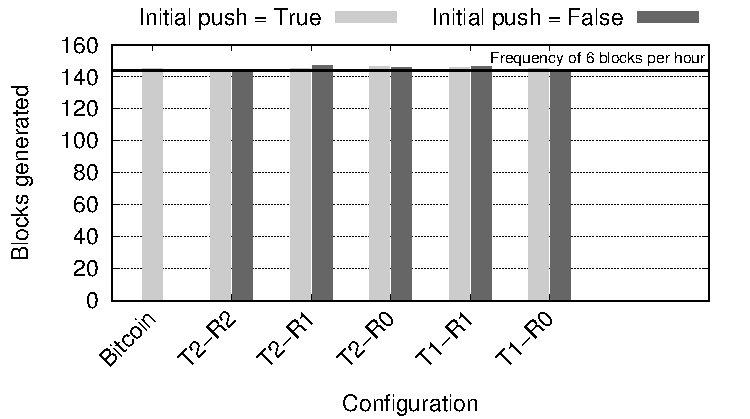
\includegraphics[width=0.5\textwidth]{plots/blocks-gen.pdf}
\caption{Blocks generated.}
\label{fig:nb-blocks}
\end{figure}

\begin{figure}
\centering
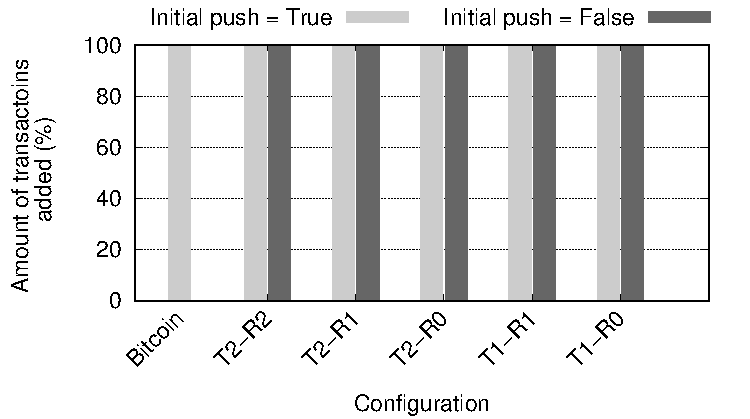
\includegraphics[width=0.5\textwidth]{plots/tx-added.pdf}
\caption{Percentage of transactions committed.}
\label{fig:tx-added}
\end{figure}

The Figure~\ref{fig:nb-blocks} shows for each configuration the amount of blocks that were generated during each experiment, meanwhile Figure~\ref{fig:tx-added} shows the percentage of transactions added to blocks. Given that we were trying to simulate a Bitcoin network, the simulator generated the expected amount of blocks for a day ($\approx 144$) and committed all the transactions created ($\approx 100\%$). This shows that for every configuration the transactions were reaching a miner and were eventually committed.

\begin{figure}[t]
\centering
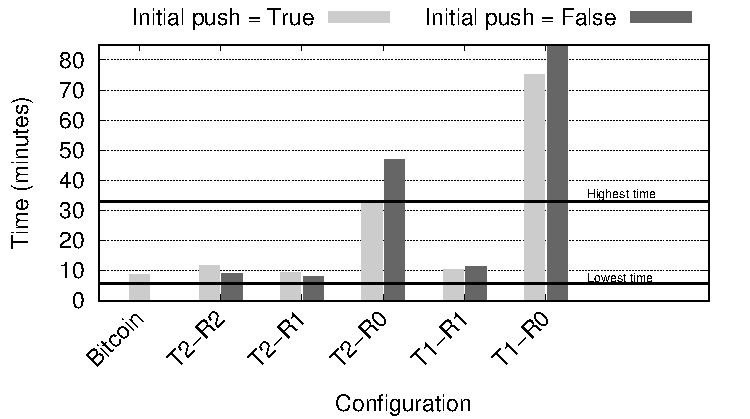
\includegraphics[width=0.5\textwidth]{plots/commit-time.pdf}
\caption{Average time it takes for a transaction to be committed.}
\label{fig:commit-time}
\end{figure}

In Figure~\ref{fig:commit-time} we measured the average time that each configuration takes for committing a transaction. The horizontal lines represent the highest average time and lowest average time it took for a transaction to be committed in Bitcoin. In this image, we can clearly see that both configurations \textsl{T2-R0} and \textsl{T1-R0} are not good enough to achieve a commit time inside the spectrum desired. This also shows that sending transactions for at least one random node alongside our top nodes has a great impact in the commit time as previously stated in Section~\ref{sec:sr}

\begin{figure}[t]
\centering
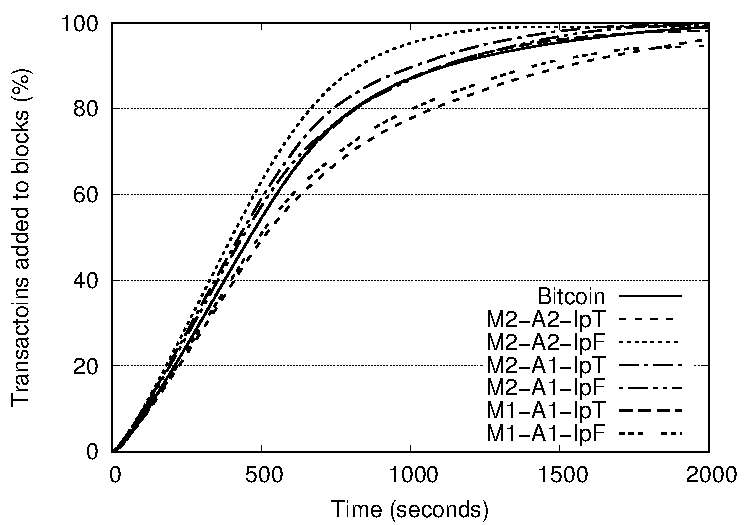
\includegraphics[width=0.5\textwidth]{plots/cdf_commit.pdf}
\caption{Cumulative distributed function of the time it takes for a transaction to be committed.}
\label{fig:cdf-commit}
\end{figure}

Figure~\ref{fig:cdf-commit} shows the cumulative distributed function of the time took to commit all the transactions, hence, is a different perspective of Figure~\ref{fig:commit-time}. We can also observe in this two images that after creating a transaction sending it to all our neighbours (\emph{ip=T}) has a very low impact in the time it takes to commit a transaction. This probably happens because the time, it takes for a transaction to reach all the miners, is lower than the rate at which blocks are being generated.

Having analysed the impact of our approach in terms of observable effects in the network like how much time it takes for a transaction to be added to a block and amount of transactions committed we will now focus on the savings in terms of messages sent and in the amount of information transmitted.
\begin{figure}[t]
\centering
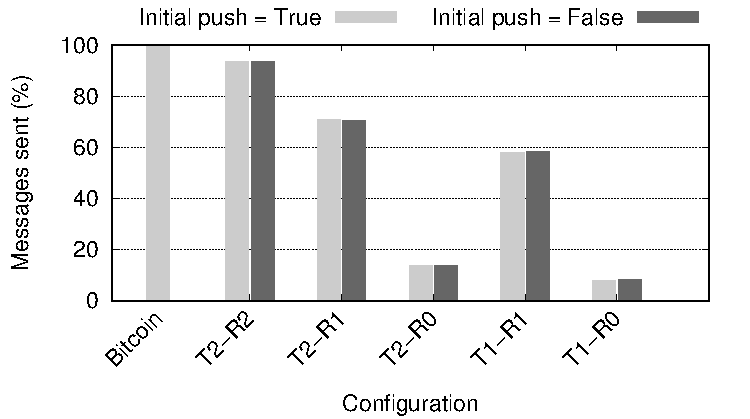
\includegraphics[width=0.5\textwidth]{plots/msg-sent.pdf}
\caption{Total number of messages sent.}
\label{fig:msg-sent}
\end{figure}

\begin{figure}[t]
\centering
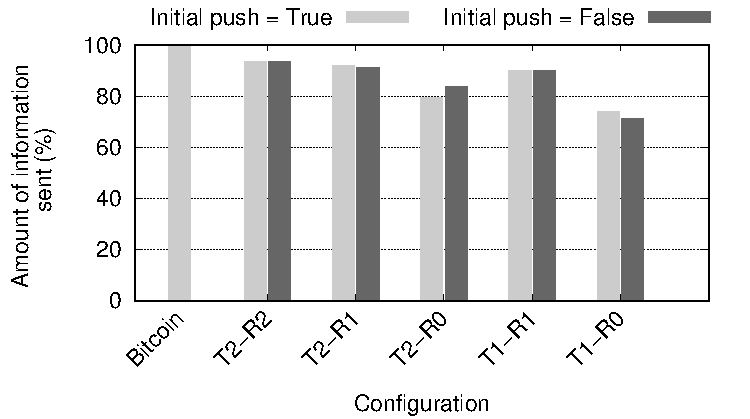
\includegraphics[width=0.5\textwidth]{plots/mb-sent.pdf}
\caption{Amount of information sent.}
\label{fig:mb-sent}
\end{figure}

In Figure~\ref{fig:msg-sent} we can see the total number of messages sent in percentage to the amount that it was sent on the Bitcoin network. As expected the configurations with a higher amount of savings were the configurations that did not relay to random nodes. This happens because when we send a transaction to a random node there is a higher chance that that node still does not have that transaction and will request it. Unfortunately, as we have seen previously both these configurations are not viable because both take to much time to commit transactions. Figure~\ref{fig:mb-sent} shows the percentage of the total amount of information, as expected, it follows a similar pattern to Figure~\ref{fig:msg-sent}. We can also see that the savings from Figure~\ref{fig:mb-sent} are not as big as the ones from Figure~\ref{fig:msg-sent} this happens because the advertise messages that we avoid sending are not very big in size. However, processing those messages in the real worlds always takes a toll on the nodes.

By analysing these results we can conclude that the most promising configuration is \textsl{T1-R1} with \textsl{ip=False} because not only can we achieve relevant savings (reduction in the number of messages sent in $41.5\%$ and reduction of the amount of information sent in $10.2\%$) but also it preserves the properties of the original Bitcoin.

\subsection{Skewed relay impact}
To determine the best possible configuration we used a stable network, where miners were always the same nodes. However, as we have stated previously Bitcoin is prone to network change, given that is a peer-to-peer network. So for the following results, we used Algorithm~\ref{alg:inc} referenced in Section~\ref{sec:nc}, as well as, all nodes start the simulation by sending advertisements to all their neighbours. Then throughout the simulation, the algorithm increase relay will determine the best Tn-Rn configuration for each node. We performed three experiments, one where we did not make any changes to the network, another where we change two miners in the network at 12 hours into the simulation and finally a third one where we changed all the miners at 12 hours into the simulation. With these experiments, we want to determine if our solution is able to adapt to the network preserving the commit time of the transactions while still trying to send as few messages as possible.

\begin{figure}[t]
\centering
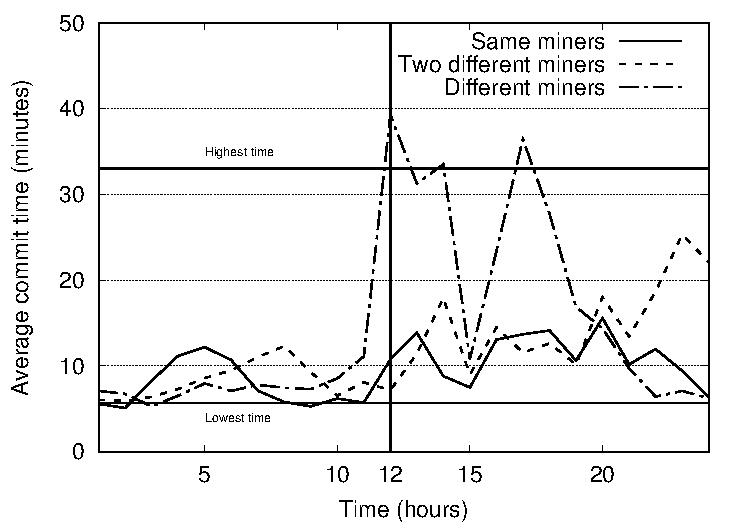
\includegraphics[width=0.5\textwidth]{plots/commit_over_time.pdf}
\caption{Average commit over time.}
\label{fig:commit-over-time}
\end{figure}

\begin{figure}[t]
\centering
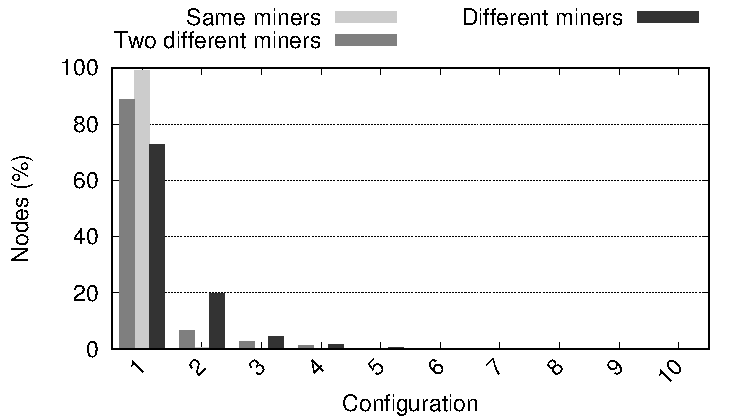
\includegraphics[width=0.5\textwidth]{plots/nodes_per_config.pdf}
\caption{Distribution of the nodes by the different possible configurations.}
\label{fig:node-per-conf}
\end{figure}

Figure~\ref{fig:commit-over-time} shows the average commit time over the period of time simulated, it also shows the two horizontal lines that were in Figure~\ref{fig:commit-time}. Figure~\ref{fig:node-per-conf} displays the percentage of nodes in each configuration at the end of the simulation for the three runs. From both of these images, we can conclude a couple of things. First, we can see that if we are in the presence of a stable network, then our solution is going to start adapting to the network and converge to the configuration that we previously deemed ideal (\textsl{T1-R1}), as seen in Figure~\ref{fig:node-per-conf}. Secondly, we can conclude that if there are slight changes to the network, then the average commit time of our solution is going to deteriorate a little bit, but soon after the algorithm will increase the size of \textsl{T} and \textsl{R} to cope with the changes and the average commit time will once again converge to more regular times. Finally, if our solution is confronted with drastic changes to the network it will not be able to maintain the current commit time, given that at 12 hours into the simulation most nodes were configured to \textsl{T1-R1} which is not resilient enough for these cases. However, eventually, our solution will start converging to the desired time. 
%Note that in our experiments we configured the most desirable configuration to be the one where we send as few messages as possible (\textsl{T1-R1}) but if for instance, we wanted to maintain the commit time in very dynamic environments then the most desirable configuration would probably be \textsl{T2-R2} as it would be more resilient against dramatic changes.

\section{Related work}
In Bitcoin, the dissemination of information is one the most important mechanisms for the network to function properly. Multiple studies have focused on analyzing the protocol of information dissemination and the problems it currently has that may lead to forks in the network ~\cite{decker2013information,croman2016scaling,miller2015discovering}.
Other works have focused on how to explore vulnerabilities in the current dissemination mechanisms in order to benefit the attacker or put the victim in a disadvantageous situation~\cite{apostolaki2016hijacking, sapirshtein2016optimal, eyal2014majority}. For instance, delay the dissemination of information could put miners at a disadvantage if the miner retaining the information already has a block mined.

However, the dissemination mechanism already has gone through multiple changes since its introduction~\cite{nakamoto2008bitcoin}. Some of these changes can be found in multiple \textsl{Bitcoin Improvement Proposals}~\cite{bip152,bips} however, we were only able to identify some of the changes done to the current client by analyzing the source code thoroughly. 

\section{Conclusions}
In conclusion, despite the multiple iterations and improvements, that have been done to the protocol of dissemination since its introduction, there are still nowadays some aspects that could be improved. Given the current size of the network and the introduction of new clients to the system is of utmost importance that the new systems are efficient without hurting the resilience of the system. In this article, we propose multiple improvements to the current algorithm of dissemination that allow us to save, 10.2\% of the current bandwidth used and 41.5\% of the number of messages exchanged.

As future work, we hope to develop an improvement to membership protocol with the help of information gathered to build more efficient paths.

%\end{document}  % This is where a 'short' article might terminate

%
% The following two commands are all you need in the
% initial runs of your .tex file to
% produce the bibliography for the citations in your paper.
\bibliographystyle{abbrv}
\bibliography{sigproc}  % sigproc.bib is the name of the Bibliography in this case
% You must have a proper ".bib" file
%  and remember to run:
% latex bibtex latex latex
% to resolve all references
%
% ACM needs 'a single self-contained file'!
%
\end{document}
